\section{Talloc context}
\label{talloc:sec:context}

A talloc context is the most important part of this library for it is
responsible for every single feature of this memory allocator. It is a logical
unit which represents a memory space managed by talloc.

From the programmer's point of view, talloc context is completely equivalent to
a pointer that would be returned by the memory routines from the C standard
library. This means that every context that is returned from the talloc library
can be used directly in functions that do not use talloc internally. For
example we can do this:

\begin{lstlisting}
char *str1 = strdup("I am NOT a talloc context");
char *str2 = talloc_strdup(NULL, "I AM a talloc context");

printf("%d\n", strcmp(str1, str2) == 0);

free(str1);
talloc_free(str2); /* we can not use free(str2) */
\end{lstlisting}

This is possible because the context is internally handled as a special
fixed-length structure called talloc chunk. Each chunk stores context meta data
followed by memory space requested by the programmer. When talloc function
returns a context (pointer), it returns in fact a pointer to the user space
part of the chunk. And when we want to manipulate with this context, the
library will transform the pointer to the user space part back to the starting
address of the chunk. This is also the reason why we were unable to use
|free(str2)| in the previous example -- because |str2| does not point at the
beginning of the allocated block of memory. This is illustrated on Figure
\ref{fig:talloc-context}.

\begin{figure}[H]
  \centering
  \setlength{\unitlength}{1cm}
\begin{picture}(4,7)
  % allocated memory box
  \put(0,7){\line(1,0){4}}
  \put(0,0){\line(1,0){4}}
  \put(0,0){\line(0,1){7}}
  \put(4,0){\line(0,1){7}}
  \put(0,0){\makebox(4,4){requested memory}}

  % context size
  \put(4.6,0){\vector(0,1){4}}
  \put(4.6,4){\vector(0,-1){4}}
  \put(4.8,0){\makebox(0,4)[l]{context size}}

  % allocated block
  \put(4.3,0){\vector(0,1){7}}
  \put(4.3,7){\vector(0,-1){7}}
  \put(4.8,4){\makebox(0,3)[l]{allocated block}}
    
  % context pointer
  \put(-1,4){\vector(1,0){1}}
  \put(-2,4.1){context}
    
  % talloc chunk box
  \linethickness{0.5mm}
  \put(0,7){\line(1,0){4}}
  \put(0,4){\line(1,0){4}}
  \put(0,4){\line(0,1){3}}
  \put(4,4){\line(0,1){3}}
  \put(0,4){\makebox(4,3){talloc chunk}}
 \end{picture}
  \caption{Talloc context}
  \label{fig:talloc-context}
\end{figure}

A type |TALLOC_CTX| is defined to identify a talloc context in function
parameters. However, this type is just an alias for |void| and exists only
for a semantical reason -- so we can differentiate between |void*| (arbitrary
data) and |TALLOC_CTX*| (talloc context).

\subsubsection{Context meta data}
Every talloc context carries several information along the code:

\begin{itemize}
  \item name -- which is used in reports of context hierarchy (section
  \ref{talloc:sec:debugging}) and to simulate dynamic type system (section
  \ref{talloc:dyn-ts})
  \item size of the requested memory in bytes -- this can be used to determine
  number of elements in arrays
  \item attached destructor -- which is executed just before the memory block is
  about to be freed (section \ref{talloc:sec:destructors})
  \item references to the context
  \item children and parent contexts -- create the hierarchical view on the
  memory
\end{itemize}

\subsection{Hierarchy of talloc contexts}

Every talloc context contains information about its parent and children. Talloc
uses this information to create a hierarchical model of memory or to be more
precise, it creates an n-ary tree where each node represents a single talloc
context. The root node of the tree is referred to as a top level context -- a
context without any parent.

This approach has several advantages:

\begin{itemize}
  \item as a consequence of freeing a talloc context, all of its children
  will be properly deallocated as well
  \item at any time, we can change the parent of a context, which
  will result in moving the whole subtree under another node
  \item it creates a more natural way of managing data structures
\end{itemize}

Let me illustrate this on an example. We have a structure that stores basic
information about a user -- his/her name, identification number and groups
he/she is a member of:

\begin{lstlisting}[caption={struct user},label={struct-user}]
struct user {
  uid_t uid;
  char *username;
  size_t num_groups;
  char **groups;
};
\end{lstlisting}

Building of such structure with talloc is very similar to the way it is done
using C standard library. We have to allocate memory for every single element of
|struct user|. The main difference is that we will specify the parent to which
the new talloc context will be attached to.

The following listing illustrates how it would be done with the C standard
library:

\begin{lstlisting}[caption={Building struct user -- C standard library}]
int i;
struct user *user = malloc(sizeof(struct user));
user->uid = 1000;
user->num_groups = N;

user->username = strdup("Test user");
user->groups = malloc(sizeof(char*) * user->num_groups);

for (i = 0; i < user->num_groups; i++) {
  user->groups[i] = asprintf("Test group %d", i);
}
\end{lstlisting}

\noindent
The following sample solves the same issue but using talloc library. We will
create a context tree that is illustrated on Figure
\ref{fig:context-tree-1-user}.

\begin{lstlisting}[caption={Building struct user -- talloc library},
label={lst:context-tree-user},
morekeywords={talloc,talloc_strdup,talloc_array,talloc_asprintf}]
/* create new top level context */
struct user *user = talloc(NULL, struct user);

user->uid = 1000;
user->num_groups = N;

/* make user the parent of following contexts */
user->username = talloc_strdup(user, "Test user");
user->groups = talloc_array(user, char*, user->num_groups);

for (i = 0; i < user->num_groups; i++) {
  /* make user->groups the parent of following context */
  user->groups[i] = talloc_asprintf(user->groups,
                                    "Test group %d", i);
}
\end{lstlisting}

\begin{figure}[H]
  \centering
  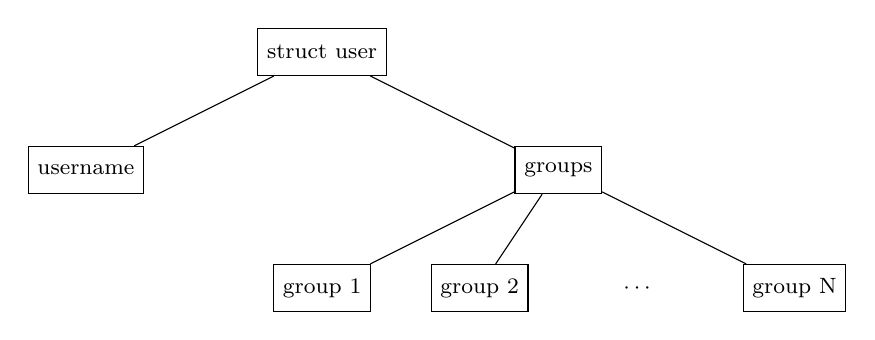
\begin{tikzpicture}
[level/.style={sibling distance=20mm},
 level 1/.style={sibling distance=60mm},
 every node/.style=
   {minimum height=6mm,rectangle,draw=black,font=\footnotesize}]
\node [] {struct user}
  child {node [] {username} }
  child {node [] {groups}
    child {node [] {group 1}}
    child {node [] {group 2}}
    child {node [draw=none] {$\cdots$} edge from parent[draw=none]}
    child {node [] {group N}}
  };
\end{tikzpicture}
  \caption{Context tree}
  \label{fig:context-tree-1-user}
\end{figure}

This way, we have gained a lot of abilities one of which is very simple
deallocation of the structure and all of its elements.

With standard C library we need to first iterate over the array of groups and
free every element separately. Then deallocate the array that stores them.
Deallocate the username and as the last step free the structure itself.

\begin{lstlisting}[caption={Freeing struct user -- C standard library},
                   label={lst:free-struct-user-c}]
int i;

for (i = 0; i < user->num_groups; i++) {
  free(user->groups[i]);
}

free(user->groups);
free(user->username);
free(user);
\end{lstlisting}

\noindent
But with talloc, the only operation we need to execute is free the structure
context. Its descendants will be freed automatically.

\begin{lstlisting}[caption={Freeing struct user -- talloc library},
                   label={lst:free-struct-user-talloc}]
talloc_free(user);
\end{lstlisting}

\subsection{Creating a new context}
\label{talloc:subsec:new-context}

Creating a new talloc context means that we want to create a new talloc chunk
(which stores the information about this context -- especially its parent and
children), allocate the desired amount of system memory and retrieve a pointer
to this memory.

Many functions exist that have the ability to create a new talloc context. This
section describes only the most fundamental ones that deal with primitive data
types and structures. Functions that are specialized in strings and arrays are
described later in this text (sections \ref{talloc:sec:strings} and
\ref{talloc:sec:arrays}).

We can divide these functions to four categories: those that allow us to set a
name of the context, functions that create a zero-length context and type safe
and type unsafe functions.

All of these functions share the following properties:
\begin{itemize}
  \item it return new talloc context or |NULL| if the system is out of memory,
  \item the first parameter is a talloc context which serves as a parent of
  the new context,
  \item the parent context can be either an existing context or |NULL| which
  will create a new top level context.
\end{itemize}

\subsubsection{Type safe functions that create a new context}

Type safe functions take as one of their parameters a data type we want to
create. It allocate the size that is necessary for this type and returns a new
properly casted pointer. This is useful if we want to rely on the compiler to
detect type mismatches.

Another feature of these functions is that they automatically set the name of
the context to the name of the data type. We can find this behaviour very handy
as it carries the type information even if we cast a variable to some other
type. We can then check for the type during the runtime as described in section
\cmplref{talloc:dyn-ts}.

The appropriate functions with this behaviour are:

\begin{funcproto}
(#type)* talloc(TALLOC_CTX *ctx, #type)
(#type)* talloc_zero(TALLOC_CTX *ctx, #type)
\end{funcproto}
\funclistend
The difference between |talloc()| and |talloc_zero()| is that the latter ensures
the whole new memory space to be initialized with zeros.

\begin{lstlisting}[caption={talloc() and talloc_zero()},label=lst:talloc_zero]
struct user *user = talloc(ctx, struct user);
if (user == NULL) {
  return ENOMEM;
}

/* initialize to default values */
user->uid = 0;
user->name = NULL;
user->num_groups = 0;
user->groups = NULL;

/* or we can achieve the same result with */
struct user *user_zero = talloc_zero(ctx, struct user);
if (user_zero == NULL) {
  return ENOMEM;
}
\end{lstlisting}

\subsubsection{Type unsafe functions that create a new context}

Type unsafe functions take as a parameter directly the size we want to
allocate instead of the type and return a pointer to |void|. The name of the
context is set to a current location in the source file where the function is
called.

If we choose to use these functions we loose both the compile-time and runtime
ability to detect a type mismatch. Therefore we should avoid using these
routines unless we really want to retrieve a |void*| (e.g. reading binary data
from a file).

The following functions are type unsafe variants of |talloc()| and
|talloc_zero()|:

\begin{funcproto}
void* talloc_size(TALLOC_CTX *ctx, size_t size)
void* talloc_zero_size(TALLOC_CTX *ctx, size_t size)
\end{funcproto}
\funclistend
There is also one very interesting macro |talloc_ptrtype(ctx, ptr)| that may or
may not be type unsafe depending on the compiler. If the compiler is |GCC| of
version greater or equal to 3, it is type safe (it uses the |__typeof__|
feature of this compiler). It is type unsafe otherwise.

It is a wrapper around |talloc_size()|, therefore the name of the context will
be the location in the source file where the macro is used. This does not depend
on whether it will be type safe or type unsafe during the compilation.

We can use it to shorten the notation if we do not need to carry the type
information in the talloc context:

\begin{lstlisting}[caption={talloc_ptrtype(ctx, ptr)},label=lst:talloc_ptrtype]
struct verylongname *x = talloc_ptrtype(ctx, x);
// instead of
struct verylongname *x = talloc(ctx, struct verylongname);
\end{lstlisting}

\subsubsection{Zero-length contexts}

Zero-length context is basically a context without any special semantical
meaning. We can use it the same way as any other context. The only difference is
that it consists only from the meta data about the context. Therefore it is
strictly of type |TALLOC_CTX*|. It is often used in case we want to aggregate
several data structures under one parent (zero-length) context.

\begin{funcproto}
TALLOC_CTX* talloc_init(const char *fmt, ...)
\end{funcproto}
\begin{funcdesc}
Creates a new top level zero-length context with a custom name.
\end{funcdesc}
\begin{funcproto}
TALLOC_CTX* talloc_new(TALLOC_CTX *ctx)
\end{funcproto}
\begin{funcdesc}
Creates a new zero-length context as a child of |ctx|. The name of the context
will be the current location in the source file prefixed with
\lstinline[showspaces=true]{"talloc_new: "}.
\end{funcdesc}

\begin{lstlisting}[caption={talloc_new()},label=lst:talloc_new]
TALLOC_CTX *ctx = NULL;
struct foo *foo = NULL;
struct bar *bar = NULL;

/* new zero-length top level context */
ctx = talloc_new(NULL);
if (ctx == NULL) {
  return ENOMEM;
}

foo = talloc(ctx, struct foo);
bar = talloc(ctx, struct bar);
\end{lstlisting}

\begin{figure}[H]
  \centering
  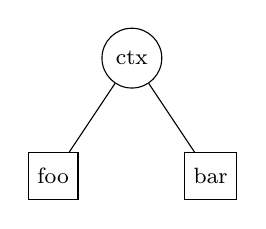
\begin{tikzpicture}
[level/.style={sibling distance=20mm},
 every node/.style=
   {minimum height=6mm,rectangle,draw=black,font=\footnotesize}]
\node [circle,draw] {ctx}
  child {node [] {foo}}
  child {node [] {bar}};
\end{tikzpicture}
  \caption{Context tree -- zero-length context}
  \label{fig:context-tree-talloc-new}
\end{figure}

\subsubsection{Contexts with custom name}

We can create a context with a custom name using the following functions: 

\begin{funcproto}
void* talloc_named(TALLOC_CTX *ctx, size_t size,
                   const char *fmt, ...)
void* talloc_named_const(TALLOC_CTX *ctx, size_t size,
                         const char *name)
\end{funcproto}
\funclistend
However, there is not much practical use for setting a custom name. These two
functions serves mainly as a generic background for the previous methods.

The only reasonable usage is to set a name of a context that is supposed to
exist for a very long time (possibly for a life time of the application). The
name will help us to identify such context during debugging. 

\subsection{Freeing a context}
\label{talloc:subsec:free-context}

There are two functions defined that deal with deallocating a context. Both
take memory context as their argument. If this context is |NULL| then no action
is performed.

\begin{funcproto}
int talloc_free(TALLOC_CTX *ctx)
\end{funcproto}
\begin{funcdesc}
  Deallocates memory occupied by the context and recursively frees its 
  children as well. The returned value is |0| on success, |-1| if |ctx| is
  |NULL| or if the destructor\footnote{More information on destructors is in
  section \cmplref{talloc:sec:destructors}} attached to this context fails.
\end{funcdesc}
\begin{funcproto}
void talloc_free_children(TALLOC_CTX *ctx)
\end{funcproto}
\begin{funcdesc}
  Frees only the children of the context.
\end{funcdesc}
\funclistend
Besides these two functions we can find useful a macro that would automatically
set the |ctx| to |NULL| to avoid accessing deallocated data. Such macro is
already defined in |talloc.h|. The name is |TALLOC_||FREE| and it is
currently defined as:

\begin{lstlisting}[caption={TALLOC_FREE(ctx)},label=lst:TALLOC_FREE]
#define TALLOC_FREE(ctx) do { \
  talloc_free(ctx);           \
  ctx = NULL;                 \
} while(0);
\end{lstlisting}

\noindent
Talloc can automatically fill the memory with some predefined character just
before the context is freed. We may want to do this to avoid reaccessing the
data after it has been deallocted -- for security reasons or to help us with
debugging of our application.

This feature is disabled by default. To enable it, we have to set
|TALLOC_FREE_FILL| environment variable. It should contain a numeric
representation of the character we want to use. For example:

\begin{lstlisting}[caption={Automatically fill the memory}]
setenv("TALLOC_FREE_FILL", "0", 1);

/* the memory occupied by ctx will be filled with '\0' "
talloc_free(ctx);
\end{lstlisting}